\documentclass{article}
\usepackage{pdfpages}
\usepackage[top=0in, bottom=0in, left=0in, right=0in]{geometry}
\usepackage{color}

\makeatletter
 \newsavebox{\@linebox}
 \savebox{\@linebox}[3em][t]{\parbox[t]{3em}{%
   \@tempcnta\@ne\relax
   \loop{ \the\@tempcnta}\\
     \advance\@tempcnta by \@ne\ifnum\@tempcnta<66\repeat}}
\makeatother

\begin{document}
\makeatletter

%% IF PAGE NUMBERS ALSO ARE NEEDED, USE \thispagestyle{plain} INSTEAD
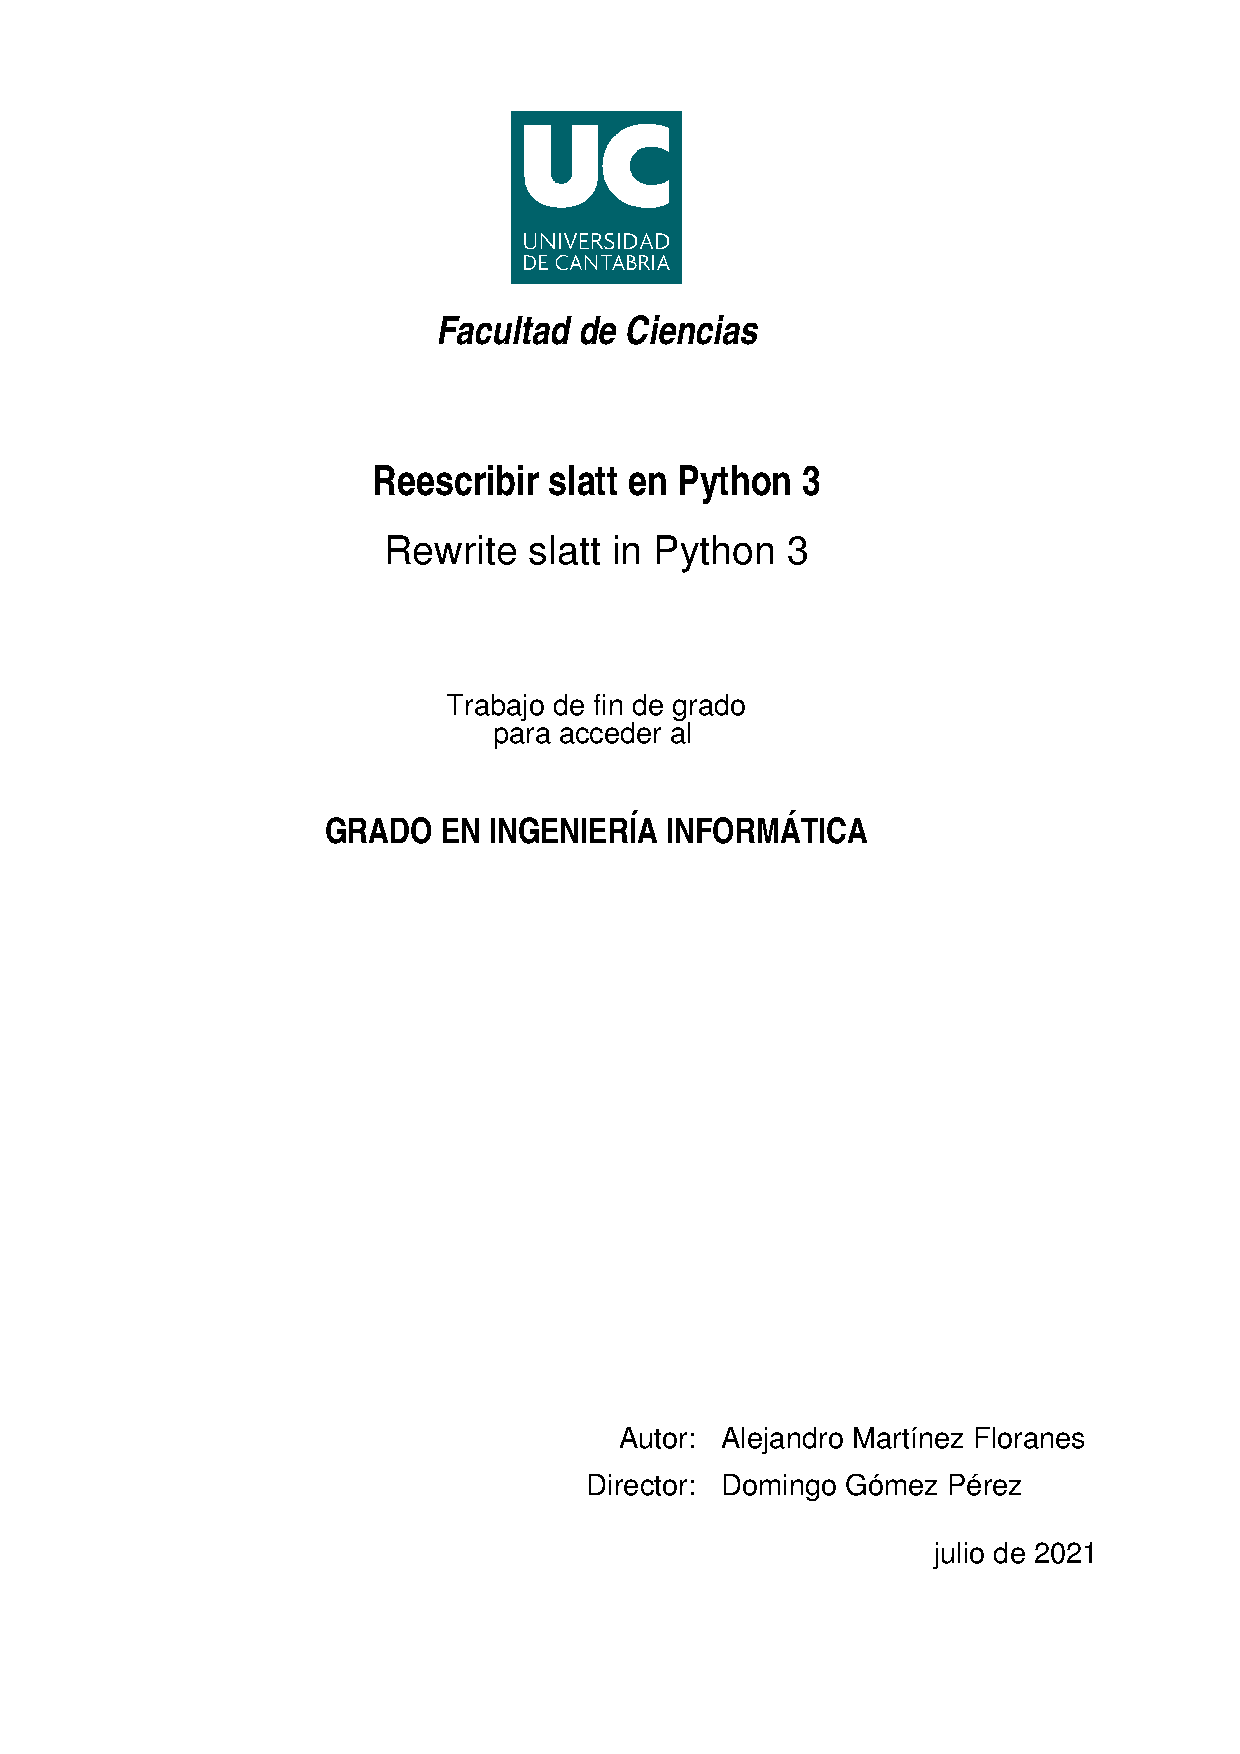
\includepdf[pages=1-,pagecommand={\thispagestyle{empty} \hspace{0.2in} \usebox{\@linebox}},fitpaper]{TFG_SLATT_python2_to_python3.pdf}

%% FOR LINE NUMBERS > 66 INCLUE OPTION openright AND DISCARD FIRST TWO PAGES OF OUTPUT
% \setcounter{page}{-1}  %% FOR LINE NUMBERS > 66 AND PAGESTYLE plain
% \includepdf[pages=1-,pagecommand={\thispagestyle{empty} \hspace{0.5in} \usebox{\@linebox}},fitpaper,openright]{loremipsum.pdf}

\makeatother
\end{document}